\chapter{Úvod}
S rozvojem moderních technologií a komunikačních zařízení se stále více aktuální stává otázka bezpečnosti a ochrany dat. Zabezpečování údajů pomocí biometrie si získalo velký úspěch, zvláště díky snadnosti přihlášení do systému a větší míře bezpečnosti jak například u~hesel. Není zde totiž potřeba si pamatovat údaje, stačí pouze použít svůj vlastní biometrický identifikátor, který bývá i bezpečnějším způsobem přihlášení nebo ochrany soukromých údajů. 

Mnoho systémů dnes využívá zabezpečení pomocí otisku prstu. Přestože tento druh identifikace se nám může jevit jako opravdu spolehlivý, i tato metoda může být napadena. Zfalšované otisky prstů mohou být vyrobeny z různých syntetických materiálů, které nemusí být nijak moc nákladné. Je proto potřeba vytvořit algoritmus, který by mohl falšování otisků prstů nějakým způsobem rozlišovat a odhalit, zda je systém narušený útočníkem.

Ve své práci se zaměřuji na implementaci kombinace různých algoritmů pro detekci živosti otisku prstu. Jedná se o algoritmy, které se zaměřují na zpracování obrazu, úpravu obrazu a výzkum, jak se dané algoritmy chovají u obrázků falešných a přirozených otisků. Pro svůj výzkum jsem využila bezdotykový senzor, který poskytuje mnoho výhod, ve srovnání s klasickámi dotykovými přístroji. Na daném senzoru probíhal sběr datasetu živých a falešných otisků prstů, kdy živé otisky mi poskytlo několik osob a falešné otisky byly vyrobeny z různých materiálů, poskytované naší fakultou. Pro práci s bezdotykovým senzorem bylo využito nasvicování prstů o světle různé vlnové délky. 

Výsledná analýza se sestávala z porovnání metod analýzy textury obrazu, analýzy hran a využití různých metod vlnkové transformace. Klasifikace probíhala za pomocí umělých neuronových sítí, algoritmu SVM a rozhodovacích stromů. Součástí mé práce je porovnání jednotlivých klasifikačních metod. Dále jsem zkoumala, jaké nasvicované světlo (červené, zelené nebo modré) vykazovalo největší přesnost a spolehlivost. 

Na souborech získaných ze senzoru jsem poté testovala implementované algoritmy, zkoumala jejich chování a vyhodnocovala závěry.




%\chapter{Abstrakt}
%\label{abstrakt}
%Pod nadpisem Abstrakt je uvedeno shrnutí práce zabírající prostor maximálně 10 řádků. Z~dobrého abstraktu by mělo být i přes jeho malý rozsah patrné, jaký problém se řešil, jaký přístup k jeho řešení byl v práci použit a jakých výsledků bylo dosaženo. Účelem abstraktu je, aby potenciální čtenář práce již po přečtení abstraktu věděl, zda v práci najde to, co hledá \cite{fitWeb}. Zbytek této kapitoly byl převzat z blogu prof. Herouta \cite{Herout}.
%\bigskip



\chapter{Biometrie} 
Biometrie je věda rozpoznávání identity člověka na základě jeho fyzických a behaviorálních vlastností jako například tvář, otisk prstů, hlas nebo oční duhovka. \cite{Jain2008} Slovo biometrie pochází z řeckých slov bios (život) a metron (měření). Biometrické identifikátory jsou v~informatice používány pro přístupovou kontrolu a identifikaci. Skoro všechny identifikátory jsou kombinací anatomických a behaviorálních charakteristik. U otisku prstu je behaviorální složkou skutečnost, že každý uživatel použije skener otisku prstů v závislosti na svém chování. Záleží i například na úhlu přiložení prstu nebo znečistění povrchu prstu či senzoru. U identifikace tváře pak záleží i na změnách pramenících z chování člověka (např. změna životního stylu vedoucí ke změně tělesné váze).\cite{Maltoni2009}
\section{Identita, identifikace, verifikace, autentizace}
Identifikace, verifikace, identita a autentizace jsou základními čtyřmi pojmy, které biometrické systémy využívají a pracuji s nimi.\cite{Drahansky}
\begin{itemize}
    \item \textbf{Identita} - Je jednoznačnou charakteristikou jedince. Rozlišujeme ji dále na:
        \begin{itemize}
            \item \textbf{Fyzická identita} - Tato identita je pouze jedna jediná. Je definována naším vzhledem a chováním.
            \item \textbf{Elektronická identita} - Těchto identit můžeme mít vytvořených nespočetně mnoho díky například více různým účtům na webové stránce.
        \end{itemize}
    \item \textbf{Identifikace} - Složí pro zjištění identity osoby. Osoba předá systému svoji biometrickou vlastnost a ten musí na základě jejího vyhodnocení rozhodnout, zda je identita nalezená nebo nenalezená. Systém k tomuto účelu používá porovnávání s databází vzorků. Jedná se o porovnání 1:N, protože se biometrická vlastnost porovnává s celou databází.
    \item \textbf{Verifikace} - Uživatel sdělí systému svoji elektronickou identitu. V systému je pak potřeba ověřit skutečná fyzická identita uživatele. Proto se hledá, zda-li jeho záznam obsahuje biometrická data. Dále se porovnává, zda sobě data odpovídají. Na základě tohoto údaje systém rozhodne o potvrzené či nepotvrzené identitě. Jedná se o porovnání 1:1, dochází k porovnání vstupních dat pouze s jedním záznamem dat v databázi.
    \item \textbf{Autentizace} - Systém při tomto úkonu potvrzuje autentičnost (hodnověrnost) dané osoby. Může být využita při identifikaci a verifikaci. Porovnávání většinou funguje na~základě pomyslného prahu.
\end{itemize}

\begin{figure}[!htbp]
    \centering
    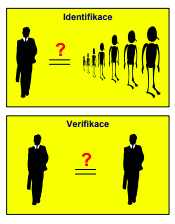
\includegraphics[width=150px]{obrazky-figures/identifver.png}
    \caption{Rozdíl mezi identifikací a verifikací, převzato z \cite{Drahansky}}
\end{figure}



\section{Biometrické systémy}
Biometrické systémy dělíme do dvou základních kategorií\cite{Drahansky}:
\begin{itemize}
    \item \textbf{Registrační modul} - Zde je zaregistrována biometrická informace (tzv. biometrický markant) a je uložena do databáze.
    \item \textbf{Verifikační modul} - Zde je zaregistrována biometrická informace podobně jako u~registračního modulu, ale výsledek není uložen do databáze, nýbrž jsou data z databáze načítána, aby se extrahovaný biometrický markant mohl porovnat s daty v~databázi. 
\end{itemize}

\begin{figure}[!htbp]
    \centering
    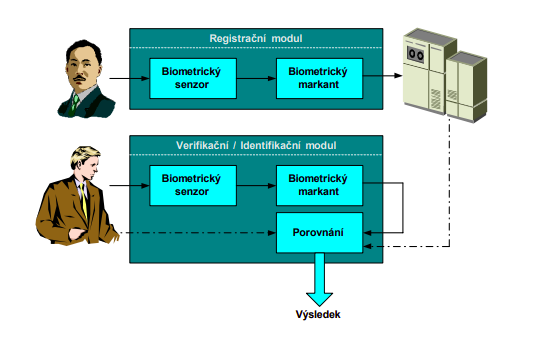
\includegraphics[width=340px]{obrazky-figures/biosystem.png}
    \caption{Znázornění biometrického systému, převzato z \cite{Drahansky}}
\end{figure}

\section{Skóre porovnání}
Skóre porovnání udává kvantifikovanou podobnost extrahovaného vzorku a šablony. Extrahovaný vzorek obsahuje významná rysy z vstupních dat. Šablona je pak uložená v např. v databázi nebo na čipové kartě. Tato míra shody je založená na aplikaci prahu T, na základě kterého je rozhodnuto o přijetí nebo nepřijetí daného objektu.\cite{Drahansky}

\begin{figure}[!htbp]
    \centering
    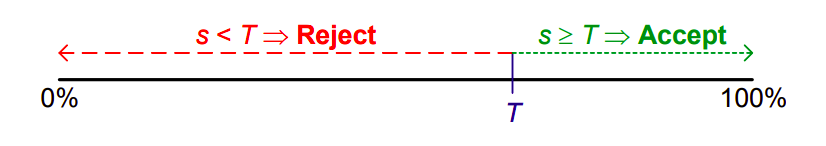
\includegraphics[width=250px]{obrazky-figures/mira.png}
    \caption{Skóre porovnání na základě zvoleného prahu, převzato z \cite{Drahansky}}
\end{figure}

\subsection{Míra chybného přijetí (FAR)}
FAR (False Acceptance Rate) udává procentuální zastoupení identifikovaných instancí, kdy jsou neautorizované osoby akceptovány daným biometrickým systémem. Tato vlastnost je spočítána následujícím vzorcem:
$$FAR = \frac{pocet\:prijatych\:neautorizovanych\:osob}{celkovy\:pocet\:testovaných\:vzorku} * 100 \%$$

\subsection{Míra chybného odmítnutí}
FRR (False Rejection Rate) představuje procentuální zastoupení identifikovaných instancí, kdy jsou autorizované osoby nekorektně biometrickým systémem zamítnuty. Výpočet je obdobný jako u charakteristiky FAR.
$$FRR = \frac{pocet\:zamitnutych\:autorizovanych\:osob}{celkovy\:pocet\:testovaných\:vzorku} * 100 \%$$

\subsection{Souvislost FAR a FRR}
Vliv charakteristik FAR a FRR znázorňuje následující graf. S větší úrovní zabezpečení se snižuje FAR, čili je přijato stále méně a méně neautorizovaných osob. Naopak se zvyšuje riziko zamítnutí autorizovaných osob daným systémem. Průsečík těchto dvou křivek nese zkratku EER (Equal Error Rate) neboli česky Míra vyrovnání chyb. V tomto bodě bude chybně akceptován a chybně odmítnut stejný počet osob. Můžeme mít systém, který je více bezpečny, ale méně uživatelsky přívětivý nebo obráceně.\cite{FARFRR}

\begin{figure}[!htbp]
    \centering
    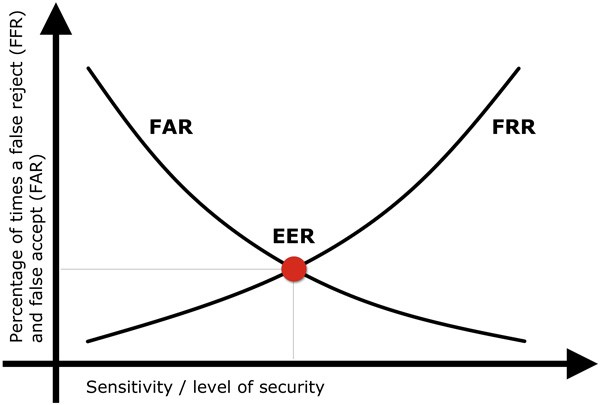
\includegraphics[width=150px]{obrazky-figures/frrfar.jpeg}
    \caption{Souvislost charakteristik FAR a FRR, převzato z \cite{FARFRR}}
\end{figure}

\chapter{Detekce otisků prstů}
\section{Historie}
Lidské otisky prstů byly objeveny na velkém počtu archeologických artefaktů a historických předmětech. I když tyto nálezy dokazují, že lidé v té době byli vědomi unikátnosti otisků prstů, až v 16. století byla objevena první vědecká technika v jejich výzkumu. V roce 1864 anglický vědec Nehemiah Grew publikoval první vědeckou studii o hřebenech, rýhách a pórech v struktuře otisku prstu.

První detailní popis struktury otisků prstů byl předveden Mayerem v roce 1788. Purkinje pak roku 1823 vytvořil první klasifikační schéma, ve kterém otisky prstů rozdělil do devíti kategorií na základě konfigurace hřebenů.\cite{Maltoni2009}

\section{Zákony daktyloskopie}
Daktyloskopie je naukou o obrazcích papilárních linií. S touto vědou se pojí samotná identifikace daktyloskopických stop a osob.\cite{PolicieDaktyloskopie} Byly zavedeny tyto daktyloskopické zákony\cite{Drahansky}:
\begin{itemize}
    \item Struktura papilárních linií je unikátní pro každého jedince.
    \item Vzor tvořený papilárními liniemi je pro každého jedince během života relativně neměnný.
    \item Obnova papilárních liní probíhá dorůstáním kůže na povrchu prstů. Mohou být pozměněny pouze pokud se poškodí nebo odstranní epidermální vrstva kůže. Poté již nemůže docházet k obnově.
    \item Konfigurační typy se mohou individuálně měnit, jedná se však o malé změny, které leží v tolerančních limitech a umožňují tak systematickou klasifikaci.
\end{itemize}

\section{Struktura otisku prstu}
Otisk prstu je tvořen vzorem papilárních linií. Výška papilárních je v rozmezí 0,1 - 0,4 mm a šířka v rozmezí 0,2 - 0,5 mm.\cite{Drahansky} Průběhy papilárních linií jsou jedinečné pro každého člověka. S přibývajícím věkem se mění rozměry plošek prstů či dlaní, avšak struktura papilárních linií zůstává stejná.

Nejvýznamější atributy papilárních liníí se vyvýjí již v nitroděložní části života. Konečná podoba papilárních linií je u dítěte již v 6. - 7. měsíci nitroděložního vývoje.\cite{DrahanskyBrezinova}

Otisky prstů dělíme na základní tři druhy:\cite{Drahansky}
\begin{itemize}
\item Válený otisk (barvený, rolovaný)
\item Píchaný otisk (živý)
\item Latentní otisk (skrytý)
\end{itemize}

\begin{figure}[!htbp]
    \centering
    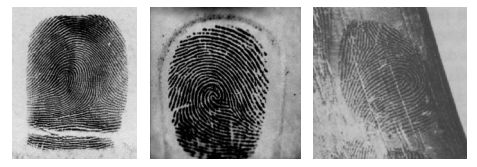
\includegraphics[width=320px]{obrazky-figures/druhyotisk.png}
    \caption{Válený, píchaný a latentní otisk prstu, převzato z \cite{Drahansky}}
\end{figure}

\section{Typy senzorů}
Nejdůležitějším částí detekce je senzor, který zaznamenává výsledný otisk prstu. Řadíme je do těchto základních kategorií:
\begin{itemize}
\item \textbf{Optické senzory} - Využívají jednoduchý zdroj světla (LED), které osvětlí plochu prstu.\cite{Drahansky} Nejvíce používaným zástupcem optických senzorů je senzor FTIR. Prst se při snímání dotýká skleněného nebo plastového hranolu. Při dotyku jsou hřebeny papilárních linií v kontaktu s povrchem snímače, ale údolí jsou vzdálena. Světlo pocházející z hranolu dopadá na prst a je odraženo údolími papilárních liníí nebo náhodně pohlceno hřebeny. Ve výsledném obrazu jsou pak hřebeny tmavá místa a údolí světlá místa. FTIR snímače dokáží snímat 3D otisk prstu a tak dokáží detekovat i zfalšované otisky prstu, které například pocházejí z fotografie. \cite{Maltoni2009}

\begin{figure}[!htbp]
    \centering
    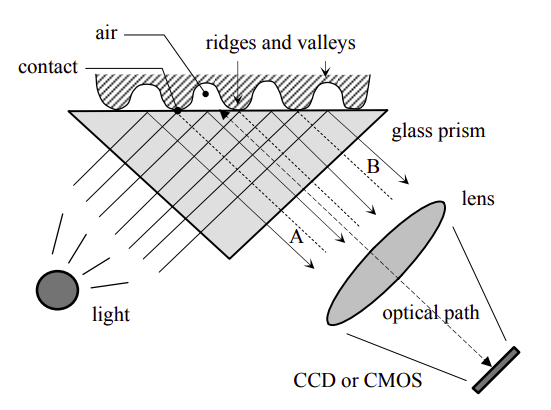
\includegraphics[width=200px]{obrazky-figures/ftiredit.png}
    \caption{Senzor FTIR, převzato z \cite{Maltoni2009}}
\end{figure}

\item \textbf{Kapacitní senzory} - Jsou složeny z matice malých vodivých plošek, na níž je napařena vrstva nevodivého oxidu křemičitého.\cite{Drahansky} Mezi povrchem prstu a každou z plošek (mikrokapacitorů) v čipu vzniká malý elektrický náboj. Při skládání výsledného otisku prstu je důležitá vzdálenost mezi povrchem otisku prstu a mikrokapacitorem. Hřebeny a údolí papilárních linií otisku prstu mají jinou vzdálenost od mikrokapacitoru, tudíž i odlišnou intenzitu ve výsledném obraze. Stejně jako u senzoru FTIR nemůže tato technologie být zneužita útočníkem při předložení fotografie. Jsou zde totiž měřeny vzdálenosti a pouze trojrozměrný povrch může být nasnímán.\cite{Maltoni2009}

\begin{figure}[!htbp]
    \centering
    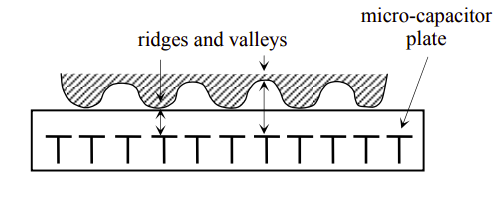
\includegraphics[width=300px]{obrazky-figures/kapacit.png}
    \caption{Kapacitní senzor, převzato z \cite{Maltoni2009}}
\end{figure}
\item \textbf{Ultrazvukové senzory} - Jsou založeny na posílání akustického signálu prstu a zachytávání odraženého signálu. Odražený signál je použit na výpočet hloubky obrazu a struktury papilárních linií. Senzor se skládá z vysílače a příjimače. Vysílač generuje krátké zvukové pulsy a příjímač detekuje odpověď po odražení těchto akustických pulsů od povrchu prstu. Senzor je schopný detekovat strukturu otisku prstu i např. přes tenké rukavice, stejně jako si dokáže poradit s nečistotami i mastnotou.\cite{Maltoni2009}

\begin{figure}[!htbp]
    \centering
    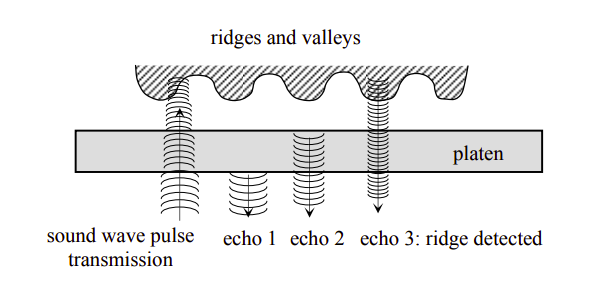
\includegraphics[width=300px]{obrazky-figures/ultrasound.png}
    \caption{Ultrazvukový senzor, převzato z \cite{Maltoni2009}}
\end{figure}
\item \textbf{Elektrooptické senzory} - Tyto snímače jsou složeny ze dvou vrstev. První dokáže emitovat světlo, pokud je polarizována správným nápětím. Druhá vrstva úzce spolupracuje s první, zpracovává emitované světlo a vytváří finální digitální obraz.\cite{Maltoni2009}\\\\\\\\

\begin{figure}[!htbp]
    \centering
    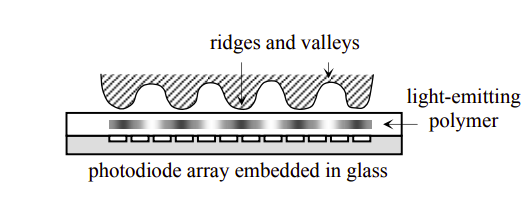
\includegraphics[width=320px]{obrazky-figures/electro.png}
    \caption{Elektrooptický senzor, převzato z \cite{Maltoni2009}}
\end{figure}
\item \textbf{Tlakový senzor} - Je vytvořen z materiálu citlivého na mechanické namáhání, při~kterém generuje elektrický signál. Velikost elektrického signálu závisí na tlaku, který vyvíjí prst na povrch senzoru. Hřebeny a údolí papilárních linií jsou v jiných vzdálenost od povrchu snímače, proto produkují jinou hodnotu elektrického signálu.\cite{Maltoni2009}
\item \textbf{Termický senzor} - Senzor využívá pyroelektrický materiál, který generuje elektrický náboj na základě teplotních rozdílů. Je založen na skutečnosti, že hřebeny v kontaktu s~povrchem senzoru produkují jinou teplotu jak údolí, které jsou vzdálenější od povrchu snímače. Senzor je obvykle předehřán na vyšší teplotu, aby se zvýšila odlišnost mezi povrchem zařízení a hřebeny linií.\cite{Maltoni2009}
\end{itemize}

\section{Základní druhy markantů}
Otisk prstu obsahuje útvary, které tvoří papilární linie - markanty. Mezi důležité markanty pro moji práci patří:
\begin{itemize}
    \item Ukončení (Line Ending)
    \item Jednoduchá vidlička (Simple Bifurcation)
    \item Dvojitá vidlička (Double Bifurcation)
    \item Trojitá vidlička (Triple Bifurcation)
    \item Hák (Hook)
    \item Křížení (Crossing)
    \item Boční kontakt (Side Contact)
    \item Bod (Point)
    \item Interval (Interval)
    \item Jednoduchá smyčka (Single Whorl)
    \item Dvojitá smyčka (Double Whorl)
    \item Jednoduchý most (Single Bridge)
    \item Dvojitý most (Twin Bridge)
    \item Průsečná linie (Through Line)
\end{itemize}

\begin{figure}[!htbp]
    \centering
    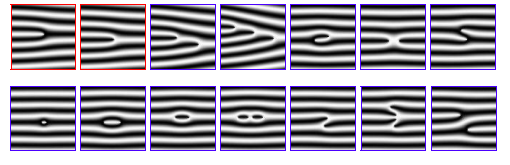
\includegraphics[width=260px]{obrazky-figures/markants.png}
    \caption{Základní typy markantů ve vyjmenovaném pořadí, převzato z \cite{Drahansky}}
\end{figure}

U přístupových systémů se však využívá pouze ukončení (Line Ending) a vidličky (Bifuraction).\cite{Drahansky}

\section{Třídy otisků prstů}
Otisky prstů můžeme na základě charakteristických znaků rozdělit do následujících kategorií:\cite{Drahansky}
\begin{itemize}
    \item Oblouk (Arch)
    \item Klenutý oblouk (Tended Arch)
    \item Spirála / závit (Whorl)
    \item Levá smyčka (Left Loop)
    \item Pravá smyčka (Right Loop)
    \item Dvojitá smyčka (Twin Loop)
\end{itemize}

\begin{figure}[!htbp]
    \centering
    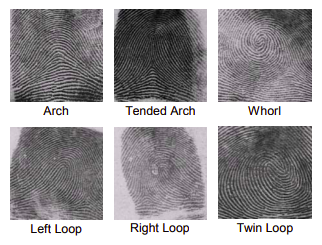
\includegraphics[width=250px]{obrazky-figures/classes.png}
    \caption{Třídy otisků prstů, převzato z \cite{Drahansky}}
\end{figure}

\section{Falšování otisků prstů}
Falešné biometrické reprezentace jsou obecně velkým nebezpečím, protože umožňují vydávat se zločinci za někoho jiného a tím narušit soukromí a bezpečnost jedince. Abnormální otisky prstů dělíme do dvou kategorií:
\begin{itemize}
    \item Falešné otisky prstů
    \item Pozměněné otisky prstů
\end{itemize}
Falešný otisk prstu reprezentuje repliku skutečného otisku prstu vyrobeného softwarově nebo z materiálů jako je želatina, silikon nebo latex. Biometrické zařízení se musí rozhodnout, zda otisk je živý nebo falešný. Tato procedura se nazývá detekce živosti.
Pozměněné otisky prstů jsou skutečné, avšak jejich struktura je změněna. Otisky mohou být neúplné, pokřivené. Důvodem poškození otisku mohou být nemoci kůže, např. pořezání, popálenina, poleptání silnými chemikáliemi, transplantace kůže a různé kožní nemoci.\cite{Petrovici}
\section{Známé metody pro analýzu živosti otisku prstu a výpočet přesnosti analýzy}
Algoritmů pro detekci živosti otisku prstu byla objevena ve studiích celá řada. Některé z nich zahrnují:\cite{AbhiskekStudy}
\begin{itemize}
    \item Použití vlastnosti elasticity lidské kůže.
    \item Umístění senzoru na zachytávání pachu vedle senzoru pro detekci otisku prstu. Senzor pachu zaznamenával výsledný signál a byl tak schopen rozpoznat lidskou kůži od~syntetických materiálů, jako např. latex, silikon nebo želatina.
    \item Kombinace statických vlastností při detekci živosti, bylo pracováno s histogramem, tloušťkou hřebenů papilárních linií, signálem detekovaným z hřebenů nebo hodnota výkonnového frekvenčního spektra.
    
\end{itemize}

Přesnost analýzy živosti $a$ můžeme spočítat na základě vzorce:
$a = \frac{C}{N}$, kde $C$ je počet správných rozhodnutí (klasifikace živého otisku prstu jako "živého" a falešného otisku prstu jako "falešného") a $N$ je počet všech rozhodnutí.\cite{GottschlichStudy}

\chapter{Bezdotykový senzor a sběr datasetu}
Tato kapitola se zabývá popisem bezdotykového senzoru, který je základním přístrojem se kterým jsem v rámci své bakalářské práce pracovala. Dále je zde popsán sběr testovacího datasetu, jak probíhalo, jak byly otisky prstů snímány a také jaké falešné otisky byly použity.

\section{Popis bezdotykového senzoru}
Bezdotykový senzor je založen na snímání, kdy daný prst nepřichází do kontaktu s žádným povrchem, jako je to u dotykových senzorů. Díky kontaktu s daným povrchem se mohou obrazy otisku prstu od stejného objektu lišit, dále je i použití dotykových senzorů otisků prstů mírně nehygienické v místech, kde ho denně použijí stovky nebo tisíce lidí. Dále jsou dané povrchy pro analýzu u dotykového senzoru ploché, ale sám povrch prstu plochý není, tudíž musí objekt použít jistý tlak na senzor, který dokáže výsledný obraz zkreslit. Bezdotykový senzor může sloužit k 2D i 3D snímání, při analýze je možné použít různé algoritmy pro analýzu textury nebo nasvícení světlem o různých vlnových délkách. \cite{PatternRecognition2006}

Použitý bezdotakový senzor v rámci bakalářské práce je složen ze tří kamer a světlech, o různých vlnových délkách, které dokáží prst nasvítit. Pro výzkum byla použita prostřední kamera. Prsty byly nasvicovány modrým, zeleným a červeným světlem. Byly provedeny experimenty i s ultrafialovým zářením, ale toto záření bylo velmi slabé a proto nebylo při výsledné práci nakonec použito.

\section{Sběr datasetu}
Pro snímky živých otisků prstů bylo použito zhruba šest osob. Prsty byly nasvicovány jednotlivými světly a bylo potřeba dbát na skutečnost, aby nebyly obrazy přesvětlené a vynikly tak co nejlépe dané papilární linie a textura povrchu prstu. I přes vynaloženou snahu, se mohou na snímcích objevit stíny, ale snažila jsem se co nejvíce simulovat skutečné používání senzoru, aby dokázal analyzovat živost s co největším rozpětím a robustností. 

Zjistila jsem, že pro některé osoby bylo zpočátku trochu nezvyklé držet prst opravdu ve statické poloze při snímání, což beru jako mírnou nevýhodu bezdotykového senzoru, kde není k dispozici žádný povrch pro položení prstu při analýze. 

Pro svoji analýzu jsem dále použila zhruba 30 falešných otisků prstů. I zde bylo potřeba dbát na co nejvyšší vyniknutí papilárních linií.

\chapter{Průzkum současných řešení detekce živosti otisků prstů}
Algoritmů pro detekci živosti otisku prstu byla objevena ve studiích celá řada. Jedná se o práce, které využívají jak hardwarové metody analýzy, tak softwarové metody. Nevýhodou hardwarových metod je, že požadují zvláštní vybavení navíc. V mojí práci se budu zabývat softwarovými metodami detekce, avšak v některých případech i s využitím hardwarového prostředku, například nasvícení prstu na senzoru světlem o různé vlnové délce. Tato kapitola popisuje stručně současné přístupy k analýze.

\section{Hardwarové metody}
Hardwarové metody využívají k určení živosti otisku prstů zvláštní hardwarová zařízení. Důležitým opatřením pro tyto metody je skutečnost, aby byly daná hardwarová zařízení integrována takovým způsobem, aby měření neohrozila kombinace útočníkova živého prstu s falešným. Těchto metod existuje celá řada, ale protože se budu spíše zabývat návrhem a práci s těmi softwarovými a nebo jejich kombinací, tak uvádím pouze některé z nich.
\subsection{Multispektrální analýza}
Kůže člověka má některé unikátní optické charakteristiky díky chemickému složení, které ovlivňuje například absorbaci optických vlastností. Díky snímcím nasvíceným světlem o různé vlnové délce, můžeme měřit různé vlastnosti lidské kůže a můžeme tedy odhalit případný falešný otisk prstu. Například modré světlo je rychle absorbováno prstem, vedle toho červené světlo prst prosvítí. Pomocí kamery je měřeno odražené světlo od nasvíceného prstu, měření může být poté vizualizováno do grafu a na základě výsledného spektra a matematických metod je stanoven výsledek.\cite{AdvancedBiometricsTechnologies2011}
\subsection{Pulsní oxyometrie}
Tato metoda využívá meření obsahu kyslíku v krvi. Využivá LED a fotodetektor na opačnýh stranách prstu. Měření závisí na srdečním tepu a proto může trvat několik sekund, než je spočten jeden nebo dva celé cykly srdečního tepu.\cite{BiometricsEncyclopedia2009}
\subsection{Teplý a studený podnět}
Lidský prst dokáže odlišně reagovat na daný podnět, který je umístěný u senzoru. Výsledná informace je zaznamenaná, konkrétně se jedná o kolísání rychlosti průtoku krve v periferních cévách. Při teplém podnětu se amplituda rychlosti toku zvyšuje, při studeném podnětu pak snižuje. Tato metoda však může být ovlivněna citlivou lidskou periferní nervovou soustavou, kdy chvíli trvá, než správně zareaguje na teplý nebo studený podnět u daného člověka.\cite{AdvancedBiometricsTechnologies2011}
\subsection{Teplota}
Teplota lidské kůže u prstu se pohybuje okolo 25 - 37 stupňů Celsia. Nicméně tento rozsah musí být širší, aby mohl systém pracovat pod různými podmínkami, i díky lidem, kteří mají problém s cirkulací krve a tato skutečnost může vést k chybným rozhodnutím při této metodě. Dalším řešením je prst zahřát. Použitím falešného otisku dosáhneme rozdílu zhruba dvou stupňů Celsia. Rozdíl je tedy malý a tato metoda není dostatečně spolehlivou pro bezpečnou detekci živosti otisků prstů.\cite{AdvancedBiometricsTechnologies2011}

\section{Softwarové metody}
Tyto metody užívají k detekci živosti informace, které jsou již obsažené v obrazu otisku prstu. Jedná se například o znaky deformace kůže, detekci pórů a další.Výhodou je, že tyto metody nemusí využívat žádné přídavné hardwarové zařízení a mohou být tedy i levnější na samotné nasazení.

\subsection{Deformace kůže a elasticita}
Tyto techniky zkoumají, jak se deformuje lidská kůže, když je prst přitlačen na povrch senzoru. Bylo zjištěno, že živé prsty se na povrchu snímače chovají způsobem, kdy se u nich projevuje značné množství nelineárního zkreslení. Falešné prsty jsou více tuhé než kůže a deformace je nižší, dokonce i když jsou falešné otisky vyrobeny z vysoce elastických materiálů.\cite{BiometricsEncyclopedia2009}

\subsection{Detekce potu}
I bříško prstu obsahuje potní žlázy, proto detekce pórů může posloužit pro detekci živosti prstu. Na základě uběhnutého času se může změřit změna velikosti pórů, kdy se vzor stává postupně tmavším. Důležitou statickou charakteristikou je pak variabilita odstínů šedi okolo hřebenů papilárních linií, dynamickou pak právě vývoj v čase při změně extrahovaného signálu z hřebenů. Falešné snímky pak nedokáží pořádně poskytnout tyto vlastnosti kvůli neschopnosti provést hlavně dané dynamické vlastnosti, které jsou u živých prstů běžné.\cite{PoresResearch}

\begin{figure}[!htbp]
    \centering
    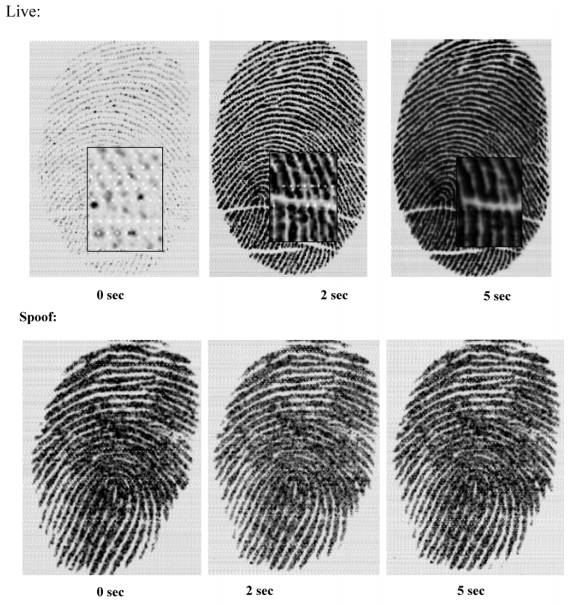
\includegraphics[width=150px]{obrazky-figures/pores.png}
    \caption{Srovnání vývoje detekce potu v čase mezi živým a falešným prstem, převzato z \cite{PoresResearch}}
\end{figure}




\chapter{Využité algoritmy pro předzpracování a analýzu živosti otisků prstů}
Tato kapitola se zabývá popisem použitých algoritmů pro předzpracování obrazu a následně vybraných algoritmů pro samotnou detekci živosti otisků prstů. Pro hlavní analýzu bylo algoritmů vybráno více, dokonce v kombinaci s některým přídavným hardwarovým vybavením. Samotná detekce se pak sestává z aplikace různých řešení a získání vlastností z samotného obrazu otisku prstu, které jsou použitelné pro rozlišení falešných a živých vzorků.
\section{Převedení na normalizovaný obraz}
Po načtení obrazu bylo potřeba obraz převést na šedotonový. Poté byla provedena normalizace obrazu. Normalizace je proces, při kterém je upraven rozsah hodnot intenzity pixelu. Základem je zvýšit dynamický rozsah šedotónového jasu, u otisků prstů tento algoritmus nemění ostrost hřebenů a údolí papilárních linií. Hlavním účelem je minimalizovat změny šedo-úrovňových hodnot podél hřebenů a údolí. 

\begin{figure}[htbp]
  \begin{minipage}[b]{0.5\linewidth}
    \centering
    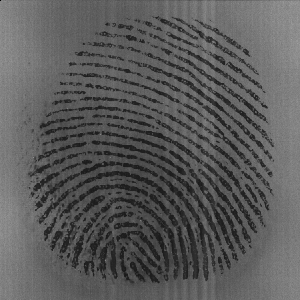
\includegraphics[width=150px]{obrazky-figures/102_1.png}
    \caption{Vstupní obraz}
  \end{minipage}
  \hspace{0.5cm}
  \begin{minipage}[b]{0.5\linewidth}
    \centering
    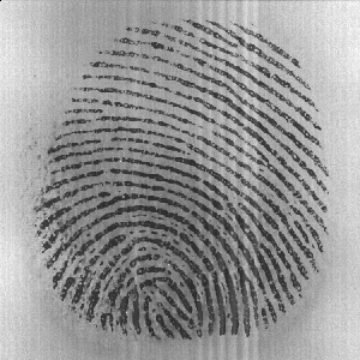
\includegraphics[width=150px]{obrazky-figures/norm_img.png}
    \caption{Normalizovaný obraz}
  \end{minipage}
\end{figure}



\section{Prahování}
Při prahování jsou světlé objekty odděleny od tmavých pomocí zadaných prahů. Tento algoritmus je nutno použít před samotnou segmentací obrazu pomocí morfologických metod. Jednoduché prahování závisí na oddělení světlých a tmavých objektů podle daných konstantních prahů. Existují však i další metody prahování, které poskytují lepší analýzu a výsledky a při mém výzkumu byly použity.

\subsection{Prahování pomocí metody Otsu}
Při globálním prahování je nutné si vybrat konstantní práh již před analýzou obrazu. Methoda Otsu tento globální optimální práh vybírá sama automaticky, na základě daného vstupního obrazu. \cite{OpenCVTresholding}Výpočet daného optimálního prahu zahrnuje iteraci přes všechny možné prahové hodnoty a výpočet rozložení pixelů na jednotlivých stranách prahu, pixelů, které spadají buď do popředí nebo pozadí obrazu. Účelem je pak najít hodnotu prahu, kdy součet rozložení na popředí a pozadí je na svém minimu.\cite{LabBookPagesTresholding}

\subsection{Adaptivní prahování}
Adaptivní prahování slouží pro analýzu obrazu např. při situacích, kdy určité části obrazu mají jiné světelné podmínky, např. při výskytu stínů. Metoda nevyužívá konstantního prahu. Algoritmus určí pro pixel hodnotu prahu na základě malého okolí okolo něj. Výsledkem jsou jiné hodnoty prahů pro různé oblasti obrazu. Pro adaptivní prahování bylo využity následující metody:\cite{OpenCVTresholding}
\begin{itemize}
    \item Adaptivní průměrné prahování (Adaptive Mean Tresholding) - Hodnota prahu je průměrem okolí. Dále je od tohoto výsledku odečtena konstanta C.
    \item Adaptivní prahování Gaussian (Adaptive Gaussian Tresholding) - Výslednou hodnotu prahu udává vážená suma okolních hodnot, kdy vahy jsou gaussian oknem. I zde je odečtena konstanta C.
\end{itemize}

\begin{figure}[!htbp]
  \begin{minipage}[b]{0.5\linewidth}
    \centering
    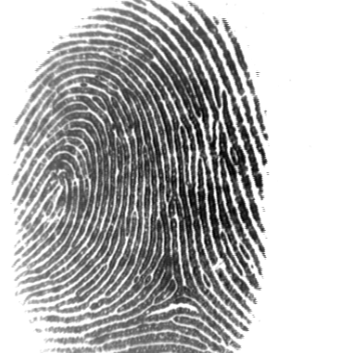
\includegraphics[width=100px]{obrazky-figures/104_7norm.png}
    \caption{Normalizovaný obraz}
  \end{minipage}
  \hspace{0.5cm}
  \begin{minipage}[b]{0.5\linewidth}
    \centering
    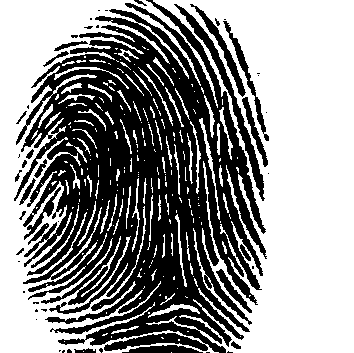
\includegraphics[width=100px]{obrazky-figures/tresh104.png}
    \caption{Obraz po aplikaci prahování}
  \end{minipage}
\end{figure}
\section{Segmentace}
Při segmentaci vybereme z vstupního obrazu pouze otisk prstu, což nám napomáhá eliminovat pozadí obrazu. Bylo využito morfologického otevření - kombinace eroze a následné diletace obrazu.

Morfologické operace se používají obvykle na úpravu binárního obrazu. Potřebují dva vstupy - náš vstupní obraz a jádro.\cite{OpenCVMorphology} Tyto operace se používají často na obrazové předzpracování - odstraňují šum a zjednodušují tvary objektů. Eroze je morfologickou operací, která je užitečná pro odstranění malých bílých částí v obraze. Diltace je opakem eroze a použivá se k zaplnění mezer.\cite{ExerciseMorphology}

Papilární linie jsou odděleny po vyprahování úzkými místy a tento algoritmus má za cíl úzká místa spojit a vytvořit tak masku, která bude určovat pozici otisku prstu v obrazu. Struktura objektu se tedy při vzniku masky zjednodušší. Výsledná maska je následně aplikována na normalizovaný obraz a je tedy vybrána pouze část obrazu, která obsahuje otisk prstu, pozadí zůstává bílé.

\begin{figure}[!htbp]
  \begin{minipage}[b]{0.3\linewidth}
    \centering
    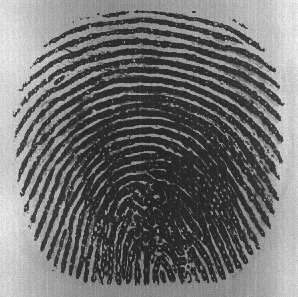
\includegraphics[width=100px]{obrazky-figures/105_5norm.png}
    \caption{Vstupní normalizovaný obraz}
  \end{minipage}
  \hspace{0.3cm}
  \begin{minipage}[b]{0.3\linewidth}
    \centering
    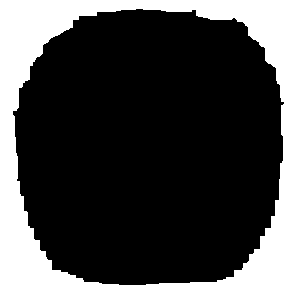
\includegraphics[width=100px]{obrazky-figures/105_5mask.png}
    \caption{Získaná maska}
  \end{minipage}
  \hspace{0.3cm}
    \begin{minipage}[b]{0.3\linewidth}
    \centering
    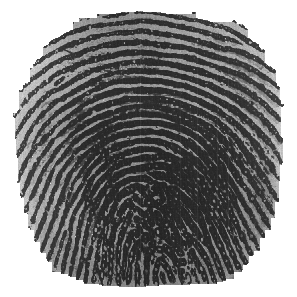
\includegraphics[width=100px]{obrazky-figures/105_5segment.png}
    \caption{Výsledný segmentovaný obraz}
  \end{minipage}
\end{figure}

%\section{Ztenčování linií}
%Pro extrakci markantů (ukončení a vidličky) je potřeba ztenčit papilární linie otisku prstů. Pro ztenčení bylo znovu využito morfologických operací. V každé iteraci algoritmu je znovu provedena eroze obrazu.
%Známým postupem pro vytvoření morfologické kostry je Lantuéjoulova formule:\cite{WikipediaSkeleton}\\\\
%Pro diskrétní binární obraz $X$ $\subset$ $\mathds{Z}^2$, skeleton $S(X)$ je sjednocením podmnožin koster ${S_n(X)},$\\$ n = 0,1,..,N$, kde:
%$$S_n(X) = (X \ominus nB) - (X \ominus nB) \circ B$$ Symboly $\ominus$ a $\circ$ jsou morfologická eroze a otevření. 

%\begin{figure}[htbp]
%  \begin{minipage}[b]{0.5\linewidth}
%    \centering
%    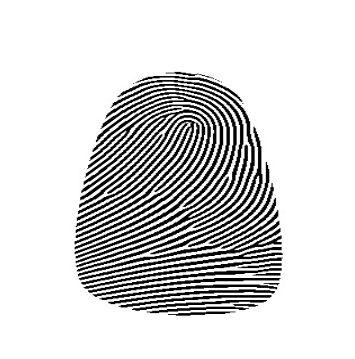
\includegraphics[width=130px]{obrazky-figures/SG_LLnorm.png}
%    \caption{Vstupní normalizovaný a segmentovaný obraz}
%  \end{minipage}
% \hspace{0.5cm}
%  \begin{minipage}[b]{0.5\linewidth}
%    \centering
%    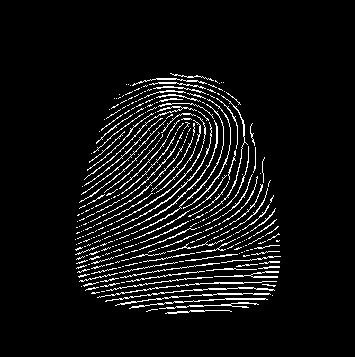
\includegraphics[width=130px]{obrazky-figures/SG_LLthin.png}
%    \caption{Obraz se ztenčenými papilárními liniemi}
%  \end{minipage}
%\end{figure}
%\section{Extrakce ukončení a vidličky}
%Extrakce těchto nejdůležitějších markantů v otisku prstu probíhá po normalizaci, segmentaci a ztenčení obrazu. Předchozí práce ukázala, že úroveň jasu v šedotónovém obrazu je náhodnou u živých otisků prstů, ale má sklon být buď uniformní nebo periodická u falešných otisků prstů. Stejná myšlenka je pak použita u místní analýzy textury otisku prstu. Z~tohoto důvodu počet hřebenů ukončení papilárních linií u živých otisků prstů má tendenci dosahovat k větším číslům, jak u falešných otisků prstů. Proto je očividné, že tato metoda může být efektivní vlastností, jak odlišit živé otisky prstů od falešných.\cite{AbhiskekStudy}

%\begin{figure}[htbp]
%    \centering
%    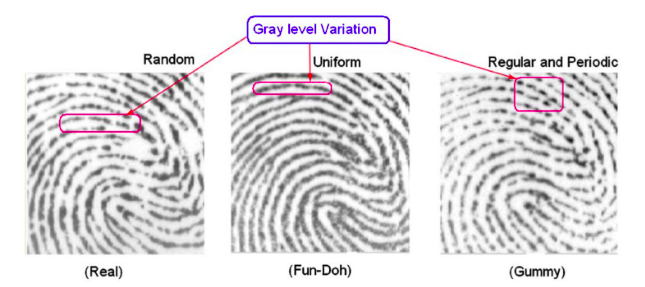
\includegraphics[width=250px]{obrazky-figures/graylevel.png}
%    \caption{Ukázka změn úrovně šedotónového jasu u živých otisků prstů v porovnání s falešnými otisky z syntetických materiálů, převzato z \cite{AbhiskekStudy}}
%\end{figure}

%Pro extrakci ukončení i vidličky bylo použito okna o velikosti 3x3 pixely. U každého pixelu pak bylo na základě tohoto okna ve středu s procházeným pixelem zjištěno, jaké hodnoty mají jeho sousedé a tento prostřední centrální pixel. 

%\begin{figure}[htbp]
%    \centering
%    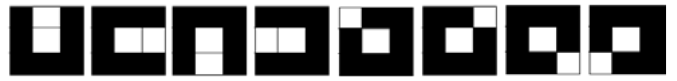
\includegraphics[width=350px]{obrazky-figures/windowridge.png}
%    \caption{Okno o velikosti 9 pixelů pro extrakci ukončení, převzato z \cite{BansalStudy}}
%\end{figure}
%\begin{figure}[htbp]
%    \centering
%    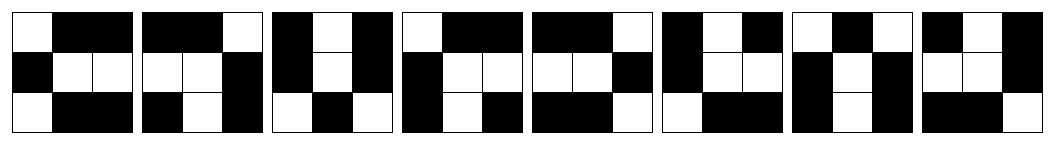
\includegraphics[width=350px]{obrazky-figures/bif.png}
%    \caption{Okno o velikosti 9 pixelů pro extrakci vidličky}
%\end{figure}





%\section{Extrakce orientovaného pole}
%Tento algoritmus z detekovaného otisku prstu vytvoří orientovanou mapu. Algoritmus postupuje následovně:\\
%1. Rozdělte normalizovaný obraz $G$ na bloky o velikosti $w$ x $w$.\\
%2. Spočítejte gradienty $\delta_x$$(i, j)$ a $\delta_y$$(i, j)$ v každém pixelu obrazu. \\
%2. Odhadněte místní orientaci každého bloku se středem v pixelu $(i, j)$ pomocí těchto rovnic:
%$$V_x(i, j) = \sum_{u=i-\frac{w}{2}}^{i+\frac{w}{2}}\sum_{v=j-\frac{w}{2}}^{j+\frac{w}{2}} 2\delta_x(u,v)\delta_y(u,v)$$
%$$V_y(i, j) = \sum_{u=i-\frac{w}{2}}^{i+\frac{w}{2}}\sum_{v=j-\frac{w}{2}}^{j+\frac{w}{2}} \delta_x^2(u,v) - \delta_y^2(u,v)$$
%$$\theta(i, j) = \frac{1}{2}\tan^{-1}(\frac{V_y(i,j)}{V_x(i, j)}$$
%3. Spočítejte magnitudu:
%$$V(i,j) = \sqrt{V_x(i,j)^2 + V_y(i,j)^2}$$
%4. Převeďte orientovaný obraz na souvislé pole vektorů pomocí rovnic:
%$$\Phi_x(i,j) = V(i,j)\cos{2\theta(i,j)}$$
%$$\Phi_y(i,j) = V(i,j)\sin{2\theta(i,j)}$$
%5. Vypočítejte výsledný úhel se středem v pixelu $(i, j)$:
%$$O(i, j) = \frac{1}{2}\tan^{-1}(\frac{\Phi_y(i,j)}{\Phi_x(i, j)}$$
%Výsledné vykreslení orientovaných úseček probíhá následovně:\\
%6. Vypočítejte počáteční body $(x_0,y_0)$ orientované úsečky:\\
%$$x_0 = i + \frac{w}{2}$$
%$$y_0 = j + \frac{w}{2}$$
%7. Vypočítejte koncové body $(x_1,y_1)$ orientované úsečky:\\
%$$r = \frac{w}{2}$$
%$$x_1 = r * \cos({O(i,j)})+ x_0$$
%$$y_1 = r * \sin({O(i,j)})+ y_0$$
%8. Sestavte výsledné rovnice orientovaných úseček. Vypočtený úhel je kolmý směrem k hřebenům papilárních linií:\\
%$$x_1 = r * cos(O(i,j)- \frac{\pi}{2}) + x_0$$
%$$y_1 = r * sin(O(i,j)- \frac{\pi}{2}) + y_0$$

%\begin{figure}[htbp]
%  \begin{minipage}[b]{0.5\linewidth}
%    \centering
%    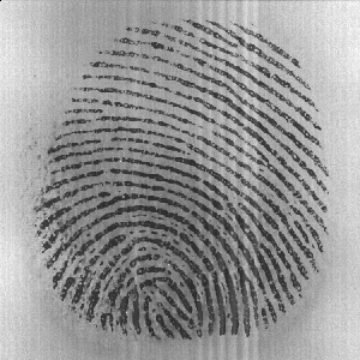
\includegraphics[width=135px]{obrazky-figures/norm_img.png}
%    \caption{Normalizovaný a segmentovaný obraz}
%  \end{minipage}
%  \hspace{0.5cm}
%  \begin{minipage}[b]{0.5\linewidth}
%    \centering
%    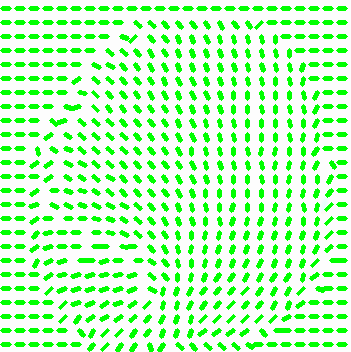
\includegraphics[width=140px]{obrazky-figures/orient.png}
%    \caption{Orientované pole obrazu}
%  \end{minipage}
%\end{figure}



\section{Lokální binární vzor}
Lokální binární vzor byl hlavním algoritmem, s jehož výstupy budu dále při práci pracovat. Jedná se o efektivní algoritmus, který se používá pro analýzu textury objektů.  Algoritmus je užitečný pro informace o změnách intenzity mezi jednotlivými pixely obrázku a jejich sousedy. Kalkulace lokálního binárního vzoru vypadá následovně:\cite{GaikwadStudy}

$$LBP(x_c,y_c) = \sum_{n=0}^{7}2^n(I_n-I(x_c,y_c)),$$
kde $I_n$ jsou hodnoty sousedních pixelů a a $I(x_c,y_c)$ hodnota středového pixelu, $n$ je index souseda.\\\\
Postup algoritmu je následující:\\
1. Pro každý pixel je zjištěno okno 3x3 pixely, kde námi procházený pixel x je středem, středem s 8 sousedy.\\
2. Pro každý pixel v 3x3 okně je spočítána nová hodnota na základě tohoto pravidla - Pokud je hodnota zjišťovaného pixelu větší nebo rovna hodnotě středového pixelu, pak je novou hodnotou zjišťovaného pixelu 1, jinak 0.\\
3. Po spočítání nových hodnot celého 3x3 okna je spočítána nová binární hodnota středového pixelu.\\

\begin{figure}[!htbp]
    \centering
    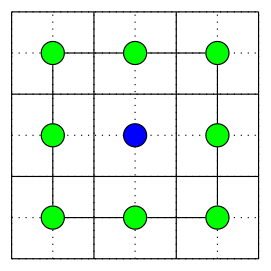
\includegraphics[width=120px]{obrazky-figures/lbpn.png}
    \caption{Okno o velikosti 9 pixelů se středovým pixelem a jeho sousedy pro analýzu lokálního binárního vzoru, převzato z \cite{GragnanielloStudy}}
\end{figure}

\begin{figure}[!htbp]
    \centering
    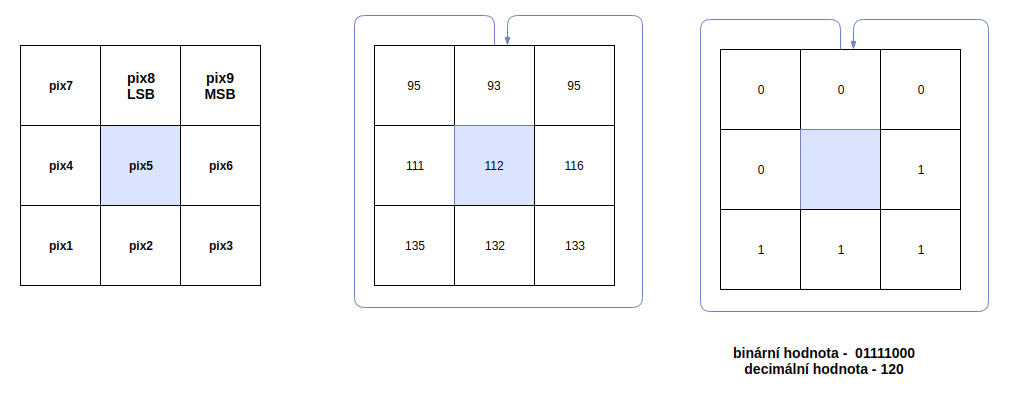
\includegraphics[width=460px]{obrazky-figures/lbpprincip.png}
    \caption{Princip výpočtu lokálního binárního vzoru, upraveno s využitím \cite{GaikwadStudy}}
\end{figure}

Pro výpočet lokálního binárního vzoru byl použit algoritmus, který lze zapsat následujícím pseudokódem:\\\\
\begin{algorithm}[H]
 \KwData{Předpracovaný obraz otisku prstu}
 \KwResult{Obraz otisku prstu zpracován LBP a výsledný histogram }
 begin\;
 \For{každý obrázek}{
    \For{každý pixel v obrazu}
    {
        zjisti pro každý pixel jeho sousední pixely v okně 3x3 vyjma krajních pixelů\;
        \For{každý pixel v okně 3x3}
        {
            porovnej každý sousední pixel s středovým pixelem\;
            \eIf{prostřední pixel > daný sousední pixel}
            {
                nastav daný sousední pixel na 1\;}
            {
                nastav daný sousední pixel na 0\;
        }
        }
    }
   vygeneruj výsledný histogram obrazu\;
  
 }
\end{algorithm}

 Nyní bylo potřeba vyextrahovat pro lokální binární vzor informace, na základě kterých by se dala detekovat problematika živosti otisku prstu. První informací, kterou jsem si z nového obrazu vyextrahovala byl jeho histogram. Histogramy se zvláště ve středových hodnotách podstatně liší. Svoji hypotézu jsem otestovala na základě porovnání částečných sum hodnot histogramů. Na základě prahu jsem pak mohla rozhodnout, zda je otisk prstu živý nebo falešný.
 
 Hypotéza byla otestována na třech databázích - dvou obsahující živé otisky prstu a jedné obsahující falešné otisky prstů. Celkem bylo pracováno se 140 snímky. Při výpočtu přesnosti budu využívat již zmiňovaný vzorec:\\
 $$a = \frac{C}{N}$$
 Do vzorce dosadíme:\\
  $$a = \frac{122}{140} = 87,14\%$$
 
 Analýzou lokálního binárního vzoru pro detekci živosti a  dalšími algoritmy se budu dále zabívat v letním semestru.
 
 %\begin{figure}[htbp]
 % \begin{minipage}[b]{0.5\linewidth}
 %   \centering
 %   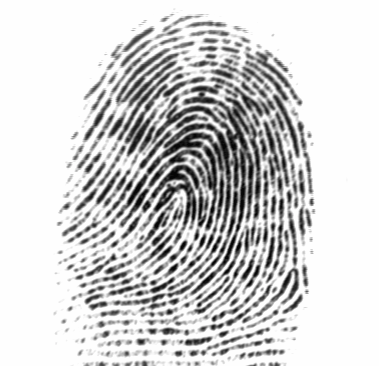
\includegraphics[width=150px]{obrazky-figures/db3.png}
 %   \caption{Snímek z databáze DB1\_B (University at Bologna)}
 % \end{minipage}
 % \hspace{0.3cm}
 % \begin{minipage}[b]{0.5\linewidth}
 %   \centering
 %   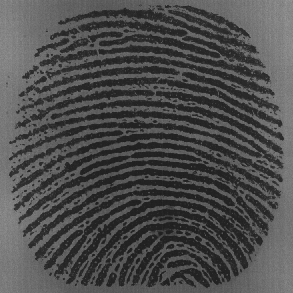
\includegraphics[width=150px]{obrazky-figures/db2.png}
 %   \caption{Snímek z databáze DB3\_B (University at Bologna)}
 % \end{minipage}
%\end{figure}
%\begin{figure}[htbp]
%    \centering
 %   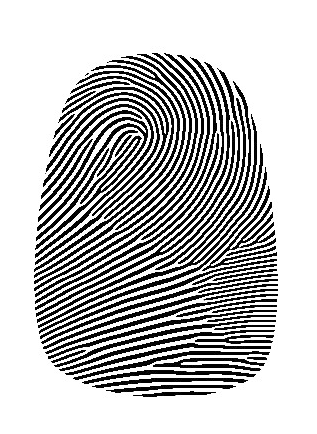
\includegraphics[width=130px]{obrazky-figures/db1.png}
 %   \caption{Snímek z obdržené databáze falešných otisků prstů}
%\end{figure}

%\begin{figure}[htbp]
%  \begin{minipage}[b]{0.5\linewidth}
 %   \centering
 %    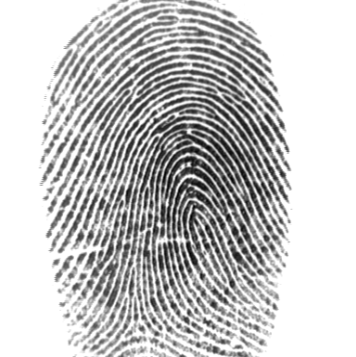
\includegraphics[width=200px]{obrazky-figures/107_7.png}
 %    \caption{Vstupní normalizovaný a segmentovaný obraz živého otisku prstu}
  % \end{minipage}
 %  \hspace{0.5cm}
  % \begin{minipage}[b]{0.5\linewidth}
  %   \centering
  %   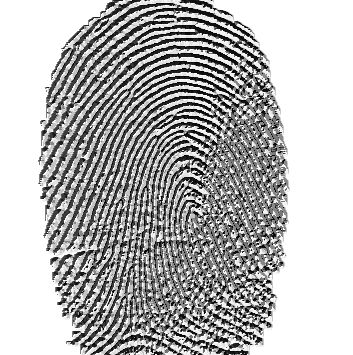
\includegraphics[width=200px]{obrazky-figures/107_7lbp.png}
 %    \caption{Výsledek aplikace lokálního binárního vzoru}
  % \end{minipage}
 %\end{figure}

 %\begin{figure}[htbp]
  % \begin{minipage}[b]{0.5\linewidth}
  %   \centering
 %    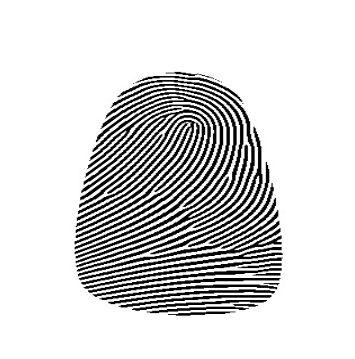
\includegraphics[width=200px]{obrazky-figures/SG_LLnorm.png}
  %   \caption{Vstupní normalizovaný a segmentovaný obraz falešného otisku prstu}
 %  \end{minipage}
  % \hspace{0.5cm}
  % \begin{minipage}[b]{0.5\linewidth}
  %   \centering
   %  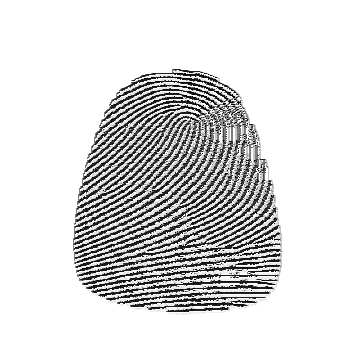
\includegraphics[width=200px]{obrazky-figures/SDLBP.png}
  %   \caption{Výsledek aplikace lokálního binárního vzoru}
  % \end{minipage}
 %\end{figure}


%\begin{figure}[htbp]
%    \centering
%    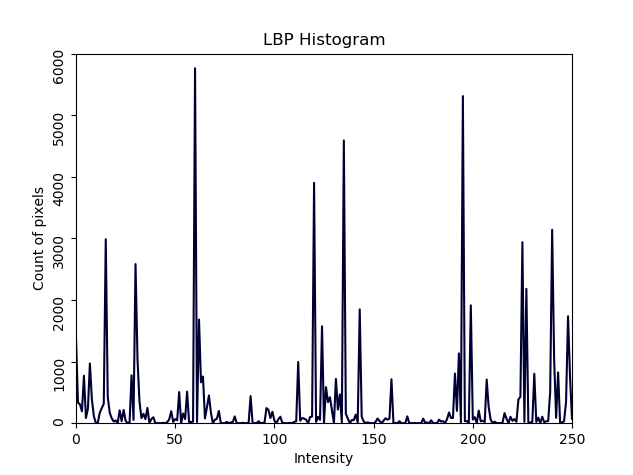
\includegraphics[width=300px]{obrazky-figures/histogramlive.png}
 %   \caption{Histogram pro výsledek lokálního binárního vzoru pro živý otisk prstu}
%\end{figure}





%
%\begin{figure}[htbp]
%    \centering
%    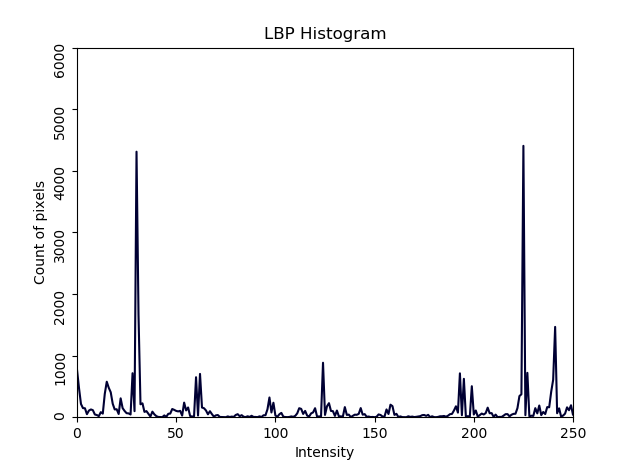
\includegraphics[width=300px]{obrazky-figures/histfake.png}
%    \caption{Histogram pro výsledek lokálního binárního vzoru pro falešný otisk prstu}
%\end{figure}

\section{Matice souvislostí stupňů šedi v obraze (GLCM)}
Matice GLCM (Grey Level Cooccurrence Matrix) slouží jako klasifikátor textury v obraze. Jedná se o čtvercovou matici, která vyjadřuje, jak často se určité kombinace hodnot pixelů v obraze vyskytují. Jedná se tedy o statistickou analýzu dané textury. Existuje až čtrnáct charakteristik, které jde z matice pro daný obraz zjistit. Pro svoji práci jsem využila čtyři z nich - kontrast, korelaci, energii a homogenitu.

Nechť $L$ x $L$ reprezentuje matici GLCM, kde prvky na souřadnicích $(i,j)$ reprezentují počet výskytů dvou sousedních pixelů, které mají hodnoty $i$ a $j$ v původním obraze. $P_{i,j}$ představuje normalizovanou matici GLCM, proměnná $levels$ dále počet stupňů šedi v obraze. Proměnné $\mu_i$, $\mu_j$, $\sigma_i$ a $\sigma_j$ charakterizují průměr a směrodatnou odchylku.\cite{TouchlessANN}

Kontrast slouží pro měření intenzity mezi pixely a jeho sousedy v celém analyzovaném obraze. Jeho rozsah je $<0, (size(GLCM,1)-1)^2>$. Kontrast o hodnotě nula představuje konstantní obraz.\cite{MatlabGLCM}\cite{ScikitGLCM}
$$contrast = \sum_{i,j=0}^{levels-1}P_{i,j}(i-j)^2$$

Korelace měří míru korelace pixelu ke svým sousedům. Nabývá hodnot v rozsahu $<-1, 1>$. Tyto koncové míry charakterizují plně negativně nebo pozitivně korelovaný obraz.\cite{MatlabGLCM}Tuto charakteristiku můžeme spočítat podle následujícího vzorce:\cite{ScikitGLCM}
$$correlation = \sum_{i,j=0}^{levels-1}[\frac{(i-\mu_i)(j-\mu_j)}{\sqrt{({\sigma_i}^2)({\sigma_j}^2)}}$$

Energie počítá s sumu čtverců jednotlivých hodnot obsažených v GLCM matici. Výsledek energie leží v intervalu $<0, 1>$. Pro konstantní vstupní obraz má energie hodnotu 1 a jinak je tato vlastnost také nazývaná jako uniformita. Energie je založená na pravidelnosti, vysoké hodnoty představují obraz, který je pravidelně uspořádán.\cite{MatlabGLCM}

S pojmem energie úzce souvisí vlastnost ASM (Angular Second Moment), který se spočítá podle této rovnice:\cite{ScikitGLCM}
$$ASM = \sum_{i,j=0}^{levels-1}P_{i,j}^2$$

Výsledná energie se pak spočte jako:\cite{ScikitGLCM}
$$energy = \sqrt{ASM}$$

Poslední extrahovanou charakteristikou byla homogenita. Tato vlastnost představuje blízkost distribuce prvků v GLCM matici ve srovnání s danou GLCM diagonálou. Homogenita může nabývat hodnot z rozsahu $<0, 1>$, kde homogenita s hodnotou jedna je typická pro diagonální GLCM matici.\cite{MatlabGLCM}\cite{ScikitGLCM}

$$homogeneity = \sum_{i,j=0}^{levels-1}\frac{P_{i,j}}{1+(i-j)^2}$$

\section{Vlnková transformace}
Vlnková transformace (Wavelet transform) je další z metod, které mohou být použity při klasifikaci živosti nebo např. při rozpoznávání. Jedná se o skupinu transformací, které se liší podle dané bázové funkce - vlnky. Zadané vlnky jsou odvozené od základní funkce - mateřské vlnky (mother wavelet). Vlnková transformace je zástupcem lineární transformace. Signál (obraz) se analyzuje pomocí násobení funkcí okna a ortogonálním rozkladem, podobně jako dalších integrálních lineárních transformací. 

Vlnková transformace může být využita také pro kompresi obrazu nebo pro filtraci šumu. \cite{WaveletHlavac} Obecně představuje alternativu ke krátkodobé Fourierově transformaci. Fourierova transformace byla velmi využívána v minulosti, ale nyní se více zaměřuje na víceměřítkové transformace (Multiresolution Transform - MT), ke kterým patří i vlnková transformace. Fourierova transformace využívá pro rozklad signálu do spektrální roviny periodické sinusové a kosinusové funkce, báze vlnkové transformace je tvořena časově omezenými funkcemi - vlnkami. Vlnky mohou být nadefinovány podle charakteru analyzovaných dat a můžeme dosáhnout i velmi přesné lokalizace průdkých změn v signálu a lepšího vyhodnocení v případě nestacionárních a neperiodických signálů.\cite{WaveletElektrorevue}

\subsection{Rodičovské a dceřinné vlnky}
Mateřská vlnka je základní vlnkovou funkcí. Určuje tvar vlnky a pokrývá celý definiční obor, který nás zajímá. Mateřskou vlnku značíme symbolem $\Psi$. Má nulovou střední hodnotu.

Otcovská vlnka pak poskytuje funkci určující měřítko, tvoří z základní vlnky další s různým měřítkem a dovoluje vyjádřit detaily aproximované funkce, které zkoumáme. Otcovská vlnka se značí symbolem $\Phi$.

Odvozené vlnky nazýváme dceřinnými vlnkami. Tyto vlnky se odvozují od rodičovských vlnek za pomocí generující bázové funkce $\Psi_{s,\tau}$, kde parametr $s$ určuje měřítko vlnkové funkce a $\tau$ pak posun dané vlnkové funkce.\cite{WaveletHlavac}

\subsection{Spojitá vlnková transformace}
Spojitá vlnková transformace (Continuous Wavelet Transform - CWT) lze zapsat následující rovnicí:\cite{WaveletMathworks}
$$y(a,b) = \frac{1}{\sqrt{a}}\int_{-\infty}^{\infty} x(t)\Psi^*(\frac{t-b}{a}) dt$$
Signál $x(t)$ je korelován s vlnkami, které jsou odvozené od mateřské vlnky $\Psi(t)$. Symbol $*$ je pak značením komplexně sdružené funkce. Výsledkem je funkce $y(a,b)$, kde parametr $a$ určuje umístění vlnky na časové ose a parametr $b$ pak měřítko. Konstanta $\frac{1}{\sqrt{a}}$ pak slouží pro normalizaci energie vlnky při změnách měřítka.

Pro případ symetrické vlnkové funkce se postupně hledá míra korelace (podobnosti) mezi naším vstupním signálem a vlnkou s měnícím se měřítkem. Ve výsledku se tedy můžou extrahovat různě velké detaily z dat, které jsou zpracována.\cite{WaveletElektrorevue}

\subsection{Diskrétní vlnková transformace}
Diskrétní vlnková transformace (Discrete Wavelet Transform - DWT) pro svoje fungování nepotřebuje nadbytečné množství koeficientů, které produkuje právě spojitá vlnková transformace, ale koeficienty redukuje. Používají se koeficienty, které odpovídají měřítkům $s = 2^j$, kde parametr $j$ může nabývat hodnot z množiny $\{0,1,2,..n\}$ Díky vhodné dvojkové závislosti paramterů $s$ a $p$ můžeme vytvořit z vlnky $\Psi$ ortonormální bázi. Nechť parametry $j, k \in Z$, pak pro $s$ a $p$ platí:
$$s = 2^j$$
$$p = k2^j$$

Pak mužeme vzorec diskrétní vlnkové transformace napsat následujícím způsobem:
$$\Psi_{j,k} = \frac{1}{\sqrt{2^j}}\Psi\frac{n-k2^j}{2^j}$$

Diskrétní vlnková transformace při zpracování obrazu se využívá hlavně pro detekci hran a textur, kompresi, filtraci šumu a získání důležitých vlastností pro další klasifikaci.\cite{WaveletElektrorevue}

\section{Wavelet rodiny vhodné pro diskrétní vlnkovou transformaci v analýze obrazu}
Existuje mnoho druhů mateřských vlnek. Na základě mateřské vlnky můžeme odvodit celou danou rodinu. Vlnky mají různé vlastnosti, které můžou být např. následující:\cite{PyWaveletsBrowser}
\begin{itemize}
    \item Symetričnost
    \item Asymetričnost
    \item Ortogonálnost - Jedná se o vlnku, jejíž vlnková transformace je ortogonální, to znamená, že inverzní vlnková transformace je sdružená vlnkové transformaci.\cite{WaveletBasics} 
    \item Biortogonálnost - Vlastnost vlnky, kdy je daná vlnková transformace invertovaná, ale ne nutně ortogonální. 
\end{itemize}

Pro diskrétní vlnkovou transformaci se používají například následující Wavelet rodiny.

\subsection{Vlnky Daubechies}

Jedná se o asymetrické, ortogonální a biortogonální vlnky. Značí se jako $dbA$, kde $A$ vyjadřuje počet nulových momentů. Pro práci můžeme využít Daubechies $db1$ až $db20$, běžně užívány jsou však vlnky typu $db1$ až $db10$.\cite{PyWaveletsBrowser} Dosahují vysoké míry komprese. Poskytují stejné parametry filtrů pro přímou i zpětnou transformaci, zajišťují rychlou a přesnou rekonstrukci.\cite{WaveletHlavac} 
    
Každá Daubechies vlnka má počet nulových momentů rovných polovině svých koeficientů. Například vlnka $db1$ (také jinak zvaná jako Haar vlnka) má jeden nulový moment, $db2$ pak dva nulové momenty, atd. Nulový moment určuje schopnost vlnky reprezentovat chování polynomu nebo informace v signálu. Například vlnka $db1$ s jedním nulovým momentem snadno kóduje konstatní složky signálu. Daubechies vlnka $db2$ snadno pracuje s konstantními a lineárními signálovými složkami, $db3$ pak pracuje s konnstantními, lineárními a kvadratickými složkami signálu.\cite{WaveletsSignalImageProcessing}
    
\subsection{Biortogonální spline vlnky}
Biortogonální spline vlnky jsou symetrické, biortogonální, ale nejsou ortogonální. Pro analýzu můžeme využít vlnky $bior1.1$, $bior1.3$, $bior1.5$, $bior2.2$, $bior2.4$, $bior2.6$, $bior2.8$, $bior 3.1$, $bior3.3$, $bior3.5$, $bior3.7$, $bior3.9$, $bior4.4$, $bior5.5$ a $bior6.8$.\cite{PyWaveletsBrowser} Jinak se také nazývají Cohen–Daubechies–Feauveau vlnky. Liší se vlastnostmi a tvarem od vlnek Daubechies, ale princip konstrukce vlnek je podobný. Biortogonální spline vlnky jsou generovány pomocí B-splinu. \cite{GeneralizedBiorthogonalDaubechiesWavelets} Jsou využity ve standardu komprese obrazu JPEG 2000, dále se používají například při kompresi otisků prstů pro FBI. 
\subsection{Reverzní biortogonální spline vlnky}
Reverzní biortogonální spline vlnky jsou symetrické. biortogonální a nejsou ortogonální. Pro práci můžeme využít tyto vlnky z dané rodiny - $rbio1.1$, $rbio1.3$, $rbio1.5$, $rbio2.2$, $rbio2.4$, $rbio2.6$, $rbio2.8$, $rbio3.1$, $rbio3.3$, $rbio3.5$, $rbio3.7$, $rbio3.9$, $rbio4.4$, $rbio 5.5$ a $rbio6.8$.\cite{PyWaveletsBrowser} Tato rodina vlnek byla v minulém výzkumu využita například pro rozpoznávání oční duhovky.\cite{IrisRecognition}




\chapter{Klasifikační algoritmy pro rozhodování o živosti a neživosti otisku prstu}
Pro samotné rozhodnutí o živosti či neživosti otisku prstu je potřeba navrhnout a použít některý z klasifikátorů, které jsou založeny na bázi umělé inteligence. Pro vlastní výzkum jsem použila neuronovou síť a klasifikátor SVM (Support Vector Machine). Tato kapitola popisuje stručný úvod do umělé inteligence a popisy jednotlivých přístupů.

\section{Umělá neuronová síť}
Umělá neuronová síť byla sestavena jako abstrakce podobná lidskému myšlení. Umělý neuron se nazývá perceptron a byl inspirován právě nervovou buňkou - neurononem. Výstupní signály umělých neuronů jsou statické, narozdíl od těch skutečných. Obecné schéma umělého neuronu je následující, proměnná $u$ představuje vnitřní potenciál, $f$ pak bázovou funkci, $g$ aktivační funkci, $i$ hodnotu daného vstupu a $w$ váhu:

\begin{figure}[!htbp]
    \centering
    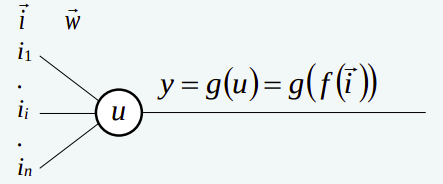
\includegraphics[width=300px]{obrazky-figures/neuron.png}
    \caption{Obecný model umělého neuronu, převzato z \cite{PrednaskaIZU9}}
\end{figure}

Každá neuronová síť funguje na následujícím principu: váhy se vynásobí s daným vstupem, dále probíhá přičtení speciální hodnoty zvané bias. Poté se aplikuje daná aktivační funkce a vstup se předá další vrstvě, zpětně se pak provádí zpětná propagace, při které se aktualizují váhy. Vnitřní stav sítě můžeme tedy charakterizovat následujícím předpisem: $w_0x_0 + \sum_{i=1}^{n}P_{i,j}w_ix_i$, kde bias představuje prvek s hodnotou $x_0$ a s vahou $w_0$ a proměnné $x_1, x_2, ...x_i$ představují vstupní hodnoty s danými vahami $w_1, w_2, ...w_i$. V některých případech může být výstup daných hodnot velmi velký, pokud pracujeme s více vrstvami neuronové sítě, hodnoty se mohou stále stávat vyššími a vyššími a samotný výpočet pak nekontrolovatelným. Proto hraje důležitou roli aktivační funkce, která na výstupu pracuje s hodnotami v určitém intervalu, např. $(-1, 1)$ nebo $(0, 1)$.\cite{MediumDeepLearning} 

V rámci bakalářské práce jsem jako aktivační funkci využila sigmoidu. Jedná se o nelineární funkci, která nabývá hodnot v intervalu $(0, 1)$, proto je vhodná pro modely, kde máme předpovědět pravděpodobnost vstupu. Rovnice funkce je následující:
$$f(x)=\frac{1}{1+e^{-x}}$$
Sigmoida je snadno diferencovatelná, můžeme ji lehce použít pro aktualizaci daných vah.

\begin{figure}[!htbp]
    \centering
    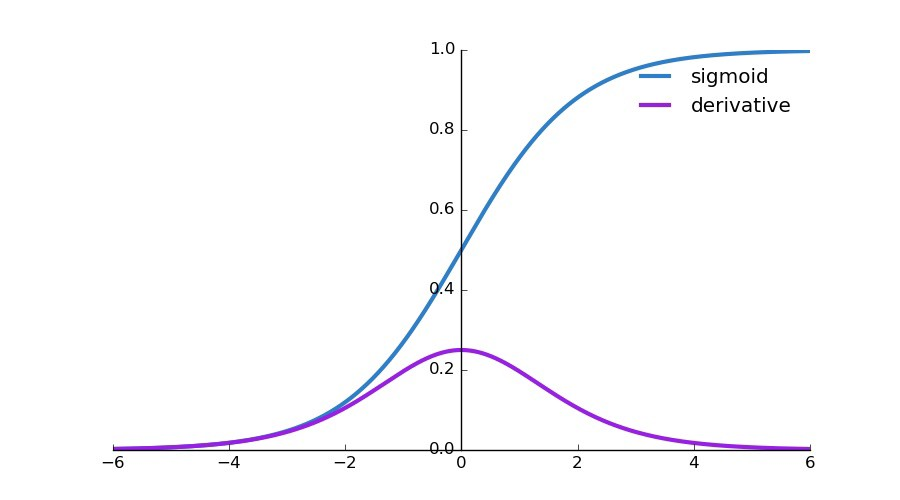
\includegraphics[width=300px]{obrazky-figures/sigmoid.jpeg}
    \caption{Graf sigmoidy a její derivace, převzato z \cite{MediumDeepLearning}}
\end{figure}

Zderivovaná sigmoida má pak následující předpis:
$$g(x)=e^{-x}*{(1+e^{-x})}^{-2}$$

Dále pro sigmoidu a její derivaci platí následující pravidlo:
$$\frac{df(x)}{f(x)} = f(x)*(1-f(x))$$

\section{Algoritmy podpůrných vektorů (SVM)}
Algoritmy podpůrných vektorů (Support Vector Machines) jsou další metodou strojového učení sloužící pro klasifikaci. Principem algoritmu je nalézt nadrovinu, sloužící pro členění daných vektorů. Data určená pro trénování, u kterých víme, jaké mají dané výsledky, jsou určena právě pro nalezení optimální nadroviny, která potom rozdělí do kategorií testované vzorky, u kterých předpovídáme výsledek. V dvourozměrném prostoru je nadrovina přímka, která dělí rovinu na dvě části (poloroviny), kdy vzorky z jedné třídy leží v jedné polorovině, vzorky druhé třídy pak v druhé polorovině. 

Pokud není možné vzorky rozumně rozdělit polorovinou, aplikujeme transformaci a přidáme jeden další rozměr, osu $z$. Nechť hodnoty bodů na ose $z$ mají hodnotu $w = x^2 + y^2$. V tomto případě můžeme měnit vzdálenosti bodu od osy $z$. Pokud nyní načrtneme graf o souřadních $yz$, vidíme zde rozdělení, které můžeme zase oddělit přímkou. 

\begin{figure}[!htbp]
    \centering
    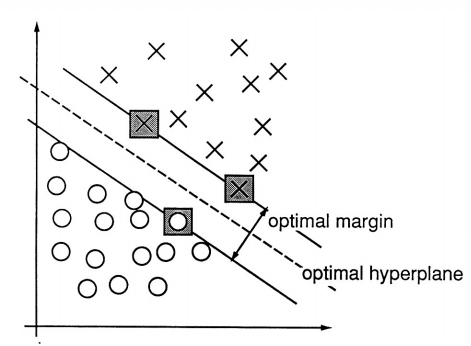
\includegraphics[width=300px]{obrazky-figures/svmVapnik.png}
    \caption{Příklad problému v dvourozměrném prostoru a nalezení optimální nadroviny a rozpětí, převzato z \cite{VapnikSVM}, na které se podílel jeden z původních výzkumníků algoritmu}
\end{figure}

\begin{figure}[!htbp]
  \begin{minipage}[b]{0.5\linewidth}
  \centering
   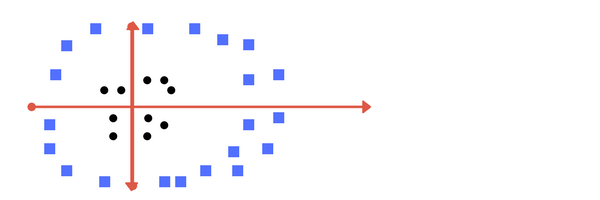
\includegraphics[width=200px]{obrazky-figures/mediumsvm1.png}
   \caption{Vstupní vzorky, které není možné rozdělit polorovinou, převzato z \cite{MediumSVM}}
  \end{minipage}
   \hspace{0.5cm}
  \begin{minipage}[b]{0.5\linewidth}
  \centering
   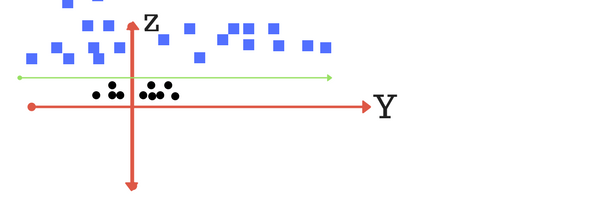
\includegraphics[width=200px]{obrazky-figures/mediumsvm2.png}
  \caption{Graf o souřadnicích yz s rozdělením na dané poloroviny, převzato z \cite{MediumSVM}} 
  \end{minipage}
 \end{figure}

Pokud zpět transformujeme tuto přímku do grafu o závislosti osy $y$ na ose $x$, vzorky jsou nyní rozděleny hranicí ve tvaru kružnice. Tato transormace se nazývá jádrová transformace. Slouží tedy pro převedení lineárně neseparovatelné úlohy na úlohu, která je již lineárně separovatelná a můžeme tedy nalézt finální rozdělující nadrovinu.\cite{MediumSVM}

\begin{figure}[!htbp]
    \centering
    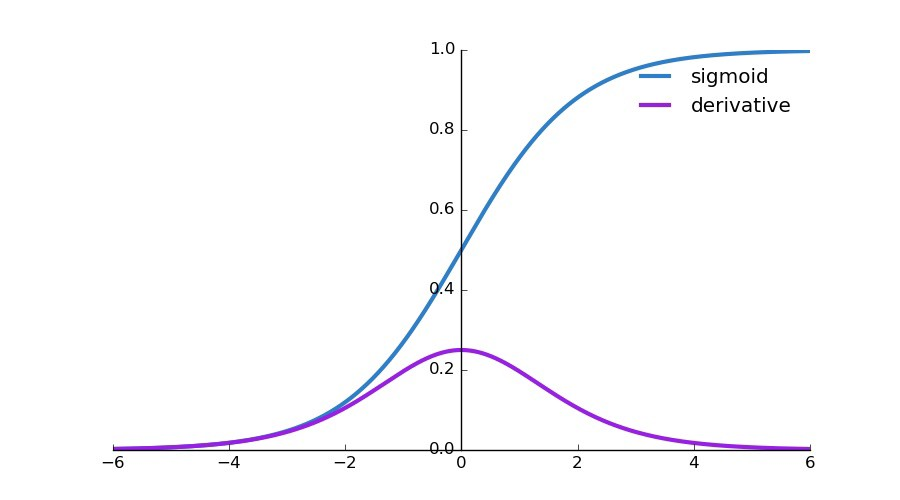
\includegraphics[width=300px]{obrazky-figures/sigmoid.jpeg}
    \caption{Nalezení finální rozdělující nadroviny, převzato z \cite{MediumSVM}}
\end{figure}

Výhodami SVM jsou:\cite{ScikitSVM}
\begin{itemize}
    \item Jedná se o efektivní metodu v prostorech o více dimenzích
    \item SVM je efektivní i při případech, kdy počet dimenzí je větší než počet vzorků
    \item Jedná se o pamětově efektivní algoritmus
\end{itemize}

Je však na druhou stranu nevýhodou, že pokud je počet vlastností o mnoho vyšší jak počet vzorků, nemusíme dostávat tolik přesné výsledky. 

\section{Rozhodovací stromy}
Cílem dalšího z klasifikačních algoritmů, rozhodovacích stromů (Decision Trees - DTs) je předpovědět výsledek na základě jednoduchých rozhodovacích pravidel, které jsou odvozené od vlastností dat. Tato klasifikační metoda tedy pro svoji práci využívá graf, který můžeme označit jako strom, protože je souvislý a neobsahuje žádnou kružnici. Cesty od kořene k listu reprezentují klasifikační pravidla. 

Výhody rozhodovacích stromů jsou:\cite{ScikitDTs}
\begin{itemize}
    \item Jednoduché na pochopení a vizualizaci, stromy jde také vizualizovat
    \item Vstupní data nemusí být různě upravována nebo normalizována
    \item Používá model white box - bílou skříňku. Pokud je daná situace v modelu pozorovatelná, vysvětlení pro podmínky může být snadno vysvětleno pomocí boolovské logiky. Umělá neuronová síť je reprezentantem modelu black box - černé skříňky, kdy mohou být výsledky obtížnější intrepretovat. 
\end{itemize}


Algoritmus však může v některých případech vytvořit až příliš komplexní strom, který data špatně zpracovává a generalizuje. Tato situace se nazývá overfitting. Jedná se tedy o chybu v modelování, kdy je model příliš složitý a fukce je příliš kompatabilní s omezenou sadou datových bodů. Při nepatrně nepřesných údajích může finální model získat podstatné chyby a predikce může být pak nepřesná.
    
\chapter{Průběh implementace, experimenty a vyhodnocení}
Cílem samotné implemetace bylo aplikovat algoritmy pro předzpracování obrazu a následně využít postupy, které mohou zajistit na základě analýzy textury výsledné rozhodnutí o živosti či neživosti daného otisku prstu.
Pro implementaci byla využit jazyk Python s dalšími podporovanými knihovnami. Pro vývoj byl využit operační systém Ubuntu 18.04.4 LTS.

\section{Knihovna OpenCV}
OpenCV je open-source knihovna, která slouží pro práci s obrazem a získávání důležitých dat. Vedle programovacího jazyka Python může být využita například i s jazykem Java nebo C++. Samotná knihovna byla napsána v jazyce C/C++.\cite{OpenCVLibrary} Vedle práce s obrazem nabízí tato knihovna například i práci s kamerami, která byla využita například při získávání dat ze senzoru. Tato knihovna byla využita při práci s otisky prstů, její funkce byly nápomocny při předzpracování obrazu a dále napomáhala i při práci při implementaci algoritmu pro lokální binární vzor.

\section{Knihovna scikit-learn}
Ekvivalentem pro knihovnu OpenCV je knihovna scikit-learn, která však umožňuje pouze podporu pro jazyk Python. Tato knihovna se primárně specializuje na podporu strojového učení, obsahuje však i funkce na podporu analýzy obrazu. Byla nápomocná při extrahování matice GLCM z obrazu, jejíž některé vlastnosti byli klíčové pro extrahovaný vektor při všech uvažovaných a zkoumaných formách analýzy. Pro klasifikaci pak byla využita funkce pro metodu SVM a taky pro rozhodovací strom. Knihovna scikit-learn představuje snadnou práci s algoritmy umělé inteligence, algoritmy jsou dobře optimalizované a rychlé. Umožňuje experimenty s různými metodami a přístupy, na základě kterých může člověk uvážit co nejvíce metod klasifikace, které mezi sebou můžeme porovnat a zkoumat chování v různých podmínkách.

\section{Knihovna PyWavelets}
Knihovna PyWavelets (pywt) představuje open source knihovnu umožňující vlnkové transformace pro práci v jazyce Python. Knihovna je částečně implementována v jazyce C. Knihovna poskytuje 1D či 2D diskrétní vlnkovou transformaci a také 1D spojitou vlnkovou transformaci. Obsahuje více jak 100 vestavěných vlnkových filtrů a podporuje i tvorbu vlastních vlnek pro uživatele. Poskytuje co nejpřesnější výsledky. Výsledky jsou kompatabilní například z Matlab Wavelet Toolbox (TM) v programovacím jazyce Matlab.\cite{PywtAbout}

\section{Implementace}

\section{Experimenty}

\section{Vyhodnocení}






\label{citace}



\chapter{Závěr}
V průběhu zimního semestru jsem se v rámci povinného předmětu Semestrální projekt (ITT) začala seznamovat s tématem detekce živosti otisků prstů. Nastudovala jsem odborné články a literaturu, začala jsem pracovat na algoritmech pro předzpracování obrazu (normalizace, prahování, ztenčování linií, extrakce orientovaného pole, extrakce markantů). Začala jsem implementovat hlavní algoritmus pro detekci živosti - lokální binární vzor. V průběhu letního semestru budu svoji práci dále rozšiřovat a zdokonalovat, chci provést výzkum nejen softwarově generovaných otisků prstů, ale i otisků prstů z různých syntetických materiálů. Plánuji navštívit laboratoř a získat snímky syntetických otisků prstů z senzoru, dále se pak chci pokusit z lokálního binárního vzoru vyextrahovat další užitečné informace kromě histogramu. Svoji detekci živosti prstu chci vedle extrakce markantů a lokálního binárního vzoru rozšířit také o práci s vlnovou délkou. Jednotlivé algoritmy poté porovnám na základě přesnosti či rychlosti zpracování. 

\label{zaver}


